\documentclass[dvipsnames,border=3pt]{standalone}
\usepackage{tikz}
\usetikzlibrary{arrows}
\usetikzlibrary{shapes}
\usepackage{enumitem}
\usepackage{bm}
\usepackage{mathdots}
\usepackage{amsmath}
\usetikzlibrary{shadings}
\usetikzlibrary{decorations.pathreplacing}
\usepackage{helvet}
\usetikzlibrary{arrows.meta}
\usepackage{graphicx}
\usepackage{pgfplots}
\usepackage{pgfplotstable}
\usepackage{filecontents}
\usetikzlibrary{plotmarks}
\usetikzlibrary{shapes.misc}
\pgfplotsset{compat=newest}

\renewcommand{\familydefault}{\sfdefault}

\definecolor{mylightgray}{cmyk}{0,0,0,0.1}
\usetikzlibrary{arrows,decorations.pathmorphing,backgrounds,fit,positioning,shapes.symbols,chains}

\begin{document}

\begin{tikzpicture}
    % trim=left botm right top
    
    \node at (4.5,2.4) {\LARGE \textbf{Correlated data with interactions}};
    
    \draw[-latex, line width=1mm,draw=gray!70] (3.62,0) -- (5.23,0);
    
    \draw[-latex, line width=1mm,draw=gray!70] (9,-1.76) -- (9,-3.4);
    %\draw[line width=1.2mm,draw=gray] (9,-2.625) -- (4.5,-2.625);
    %\draw[-latex,line width=1.2mm,draw=gray] (4.5,-2.55) -- (4.5,-3.4);
    
    \draw[-latex, line width=1mm,draw=gray!70] (0,-8.63) -- (0,-10.17);
    %\draw[line width=1.5mm,draw=gray] (4.5,-9.425) -- (0,-9.425);
    %\draw[-latex,line width=1.5mm,draw=gray] (0,-9.35) -- (0,-10.17);
    
    \draw[-latex,line width=1mm,draw=gray!70] (2.77,-11.42) -- (5.68,-11.42);
    
    %\draw[-latex, line width=1.9mm,draw=gray] (9,-1.3) -- (4.5,-3.62);
    %\node[fill=white,text height=0.2cm,text width=0.5cm] at (8.9,-1.2) {};
    %\draw[-latex, line width=1.9mm,draw=gray] (4.5,-8.295) -- (0,-10.165);
    %\node[fill=white,text height=0.2cm,text width=0.5cm] at (4.3,-8.14) {};
    %\draw[-latex, line width=1.9mm,draw=gray] (2.62,-11.42) -- (6.182,-11.42);
    
    \node at (0,0) (1) {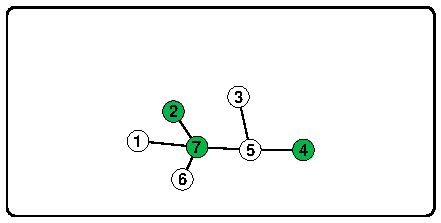
\includegraphics[clip,trim=0.1cm 0.1cm 0.1cm 0.1cm]{interaction_simulation1.pdf}};
    
    \node at (9,0) (2) {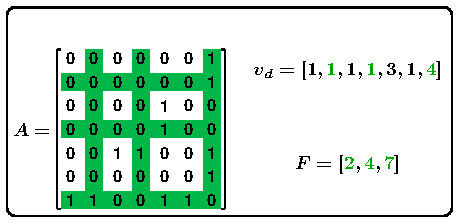
\includegraphics[clip,trim=0.1cm 0.1cm 0.1cm 0.1cm]{interaction_simulation2.pdf}};
    
    \node at (4.5,-6) (3) {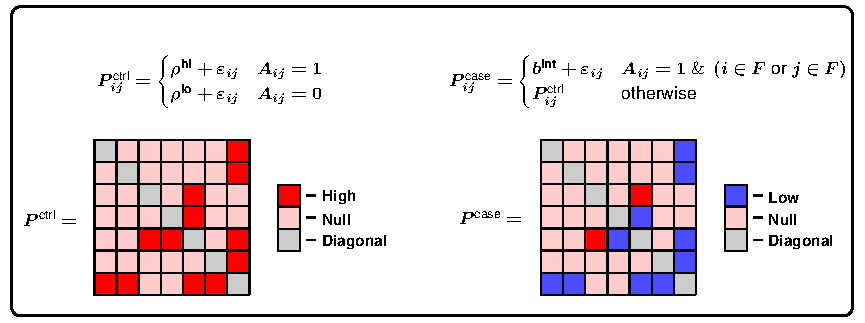
\includegraphics[clip,trim=0.1cm 0.1cm 0.1cm 0.1cm]{interaction_simulation3.pdf}};
    
    \node at (0,-11.42) (4) {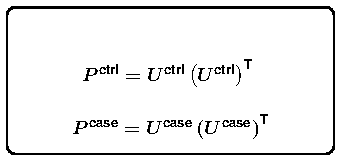
\includegraphics[clip,trim=0.1cm 0.1cm 0.1cm 0.1cm]{interaction_simulation4.pdf}};
    
    \node at (9,-11.42) (5) {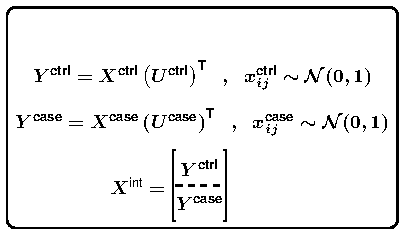
\includegraphics[clip,trim=0.1cm 0.1cm 0.1cm 0.1cm]{interaction_simulation5.pdf}};
    
    %%%%%%%%%%%%%%%%%%%%%%%%%%%%%%%%%%%%%%% box 1 %%%%%%%%%%%%%%%%%%%%%%%%%%%%%%%%%%%%%%%%%%%%%%%
    \node[circle,draw,line width=0.2mm,xscale=1.4,yscale=1.4,fill=gray!40] at (-3.3,1.45) {};
    \node at (-3.3,1.45) {\textbf{1}};
    
    \node[xscale=1,yscale=1] at (0,0.9) {\textbf{Erd\H{o}s-R\'{e}nyi or Scale-free}};
    %\node[xscale=1,yscale=1] at (2.28,0.9) {\textbf{Erdos-Renyi}};
    %\node[xscale=1,yscale=1] at (0,0.9) {\textbf{or}};
    \node[xscale=1,yscale=1] at (0,1.45) {\textbf{Random graph}};
    %%%%%%%%%%%%%%%%%%%%%%%%%%%%%%%%%%%%%%% box 1 %%%%%%%%%%%%%%%%%%%%%%%%%%%%%%%%%%%%%%%%%%%%%%%
    
    %%%%%%%%%%%%%%%%%%%%%%%%%%%%%%%%%%%%%%% box 2 %%%%%%%%%%%%%%%%%%%%%%%%%%%%%%%%%%%%%%%%%%%%%%%
    \node[circle,draw,line width=0.2mm,xscale=1.4,yscale=1.4,fill=gray!40] at (5.55,1.45) {};
    \node at (5.55,1.45) {\textbf{2}};
    
    \node[xscale=1,yscale=1] at (7.5,1.45) {\textbf{Adjacency matrix}};
    \node[xscale=1,yscale=1] at (11,1.2) {\textbf{Degree vector}};
    \node[xscale=1,yscale=1] at (11,-0.4) {\textbf{Functional features}};
    %%%%%%%%%%%%%%%%%%%%%%%%%%%%%%%%%%%%%%% box 2 %%%%%%%%%%%%%%%%%%%%%%%%%%%%%%%%%%%%%%%%%%%%%%%
    
    %%%%%%%%%%%%%%%%%%%%%%%%%%%%%%%%%%%%%%% box 3 %%%%%%%%%%%%%%%%%%%%%%%%%%%%%%%%%%%%%%%%%%%%%%%
    \node[circle,draw,line width=0.2mm,xscale=1.4,yscale=1.4,fill=gray!40] at (-2.3,-3.71) {};
    \node at (-2.3,-3.71) {\textbf{3}};
    
    \node[xscale=1,yscale=1] at (4.5,-3.64) {\textbf{Correlation matrices}};
    
    \node[xscale=1,yscale=1] at (0.1,-5.4) {\textbf{Controls}};
    \node[xscale=1,yscale=1] at (7.65,-5.4) {\textbf{Cases}};
    %%%%%%%%%%%%%%%%%%%%%%%%%%%%%%%%%%%%%%% box 3 %%%%%%%%%%%%%%%%%%%%%%%%%%%%%%%%%%%%%%%%%%%%%%%
    
    %%%%%%%%%%%%%%%%%%%%%%%%%%%%%%%%%%%%%%% box 4 %%%%%%%%%%%%%%%%%%%%%%%%%%%%%%%%%%%%%%%%%%%%%%%
    \node[circle,draw,line width=0.2mm,xscale=1.4,yscale=1.4,fill=gray!40] at (-2.45,-10.51) {};
    \node at (-2.45,-10.51) {\textbf{4}};
    \node[xscale=1,yscale=1] at (0.2,-10.48) {\textbf{Cholesky decomposition}};
    %%%%%%%%%%%%%%%%%%%%%%%%%%%%%%%%%%%%%%% box 4 %%%%%%%%%%%%%%%%%%%%%%%%%%%%%%%%%%%%%%%%%%%%%%%
    
    %%%%%%%%%%%%%%%%%%%%%%%%%%%%%%%%%%%%%%% box 5 %%%%%%%%%%%%%%%%%%%%%%%%%%%%%%%%%%%%%%%%%%%%%%%
    \node[circle,draw,line width=0.2mm,xscale=1.4,yscale=1.4,fill=gray!40] at (6.01,-9.87) {};
    \node at (6.01,-9.87) {\textbf{5}};
    \node[xscale=1,yscale=1] at (9,-9.81) {\textbf{Interaction data}};
    %%%%%%%%%%%%%%%%%%%%%%%%%%%%%%%%%%%%%%% box 5 %%%%%%%%%%%%%%%%%%%%%%%%%%%%%%%%%%%%%%%%%%%%%%%
    
\end{tikzpicture}
    
\end{document}